\documentclass[hyperref={pdftex,pdfpagemode=none,pdfstartview=FitH},10pt]{beamer}
\usepackage[english]{babel}
\usepackage{times}
%\usepackage{mathptmx,helvet}
\usepackage{amsmath,amssymb}
\usepackage{subfigure,graphicx,tabularx,booktabs,colortbl}
\usepackage{amssymb,amsmath,amsthm,times,graphicx,subfigure,tabularx,booktabs,colortbl,multirow,threeparttable,graphics}
\usepackage{movie15}
\usepackage[labelformat=empty]{caption}
\usepackage{color}
\newcommand{\hilight}[1]{\colorbox{green}{#1}}

\newcommand{\norm}[1]{\ensuremath{\left\| #1 \right\|}}
\newcommand{\bracket}[1]{\ensuremath{\left[ #1 \right]}}
\newcommand{\braces}[1]{\ensuremath{\left\{ #1 \right\}}}
\newcommand{\parenth}[1]{\ensuremath{\left( #1 \right)}}
\newcommand{\refeqn}[1]{(\ref{eqn:#1})}
\newcommand{\reffig}[1]{Fig. \ref{fig:#1}}
\newcommand{\tr}[1]{\mbox{tr}\ensuremath{\negthickspace\bracket{#1}}}
\newcommand{\trs}[1]{\mbox{tr}\ensuremath{\bracket{#1}}}
\newcommand{\deriv}[2]{\ensuremath{\frac{\partial #1}{\partial #2}}}
\newcommand{\T}{\ensuremath{\mathsf{T}}}
\newcommand{\SO}{\ensuremath{\mathsf{SO}(3)}}
\newcommand{\G}{\ensuremath{\mathsf{G}}}
\renewcommand{\d}{\ensuremath{\mathfrak{d}}}
\newcommand{\so}{\ensuremath{\mathfrak{so}(3)}}
\renewcommand{\Re}{\ensuremath{\mathbb{R}}}
\newcommand{\aSE}[2]{\ensuremath{\begin{bmatrix}#1&#2\\0&1\end{bmatrix}}}
\newcommand{\SE}{\ensuremath{\mathrm{SE(3)}}}
\newcommand{\se}{\ensuremath{\mathfrak{se}(3)}}
\renewcommand{\S}{\ensuremath{\mathbb{S}}}
\newcommand{\abs}{\mathop{\mathrm{abs}}\nolimits}


\renewcommand{\r}{\mathbf{r}}
\renewcommand{\u}{\mathbf{u}}
\newcommand{\y}{\mathbf{y}}
\newcommand{\x}{\mathbf{x}}

\definecolor{RoyalBlue}{rgb}{0.25,0.41,0.88}
\def\Emph{\textcolor{RoyalBlue}}

\definecolor{mygray}{gray}{0.9}
\definecolor{tmp}{rgb}{0.804,0.941,1.0}
\setbeamercolor{numerical}{fg=black,bg=tmp}
\setbeamercolor{exact}{fg=black,bg=red}

\mode<presentation> {
  \usetheme{Warsaw}
  \usefonttheme{serif}
  \setbeamercovered{transparent}
}

\setbeamertemplate{footline}%{split theme}
{%
  \leavevmode%
  \hbox{\begin{beamercolorbox}[wd=.5\paperwidth,ht=2.5ex,dp=1.125ex,leftskip=.3cm,rightskip=.3cm plus1fill]{author in head/foot}%
    \usebeamerfont{author in head/foot}\insertshorttitle
  \end{beamercolorbox}%
  \begin{beamercolorbox}[wd=.5\paperwidth,ht=2.5ex,dp=1.125ex,leftskip=.3cm plus1fill,rightskip=.3cm]{title in head/foot}%
    \usebeamerfont{title in
    head/foot}\insertframenumber/\inserttotalframenumber
  \end{beamercolorbox}}%
  \vskip0pt%
} \setbeamercolor{box}{fg=black,bg=yellow}

\title[Minimum Uncertainty JPDA and Coalescence-Avoiding Optimal JPDA Filtering]
{Minimum Uncertainty JPDA Filter and Coalescence
\\
Avoidance Performance Evaluations
}

\author{
Evan Kaufman\\
{\footnotesize\selectfont Department of Mechanical and Aerospace Engineering,\\
The George Washington University, Washington DC}
$ $\\
\vspace*{0.015\columnwidth}
T. Alan Lovell\\
{\footnotesize\selectfont Air Force Research Laboratory,\\ Kirtland AFB, Albuquerque NM}
$ $\\
\vspace*{0.015\columnwidth}
Taeyoung Lee\\
{\footnotesize\selectfont Department of Mechanical and Aerospace Engineering,\\
The George Washington University, Washington DC}
}


%\institute[GWU]{\footnotesize\selectfont
%$^*$ Air Force Research Laboratory, Kirtland AFB, Albuquerque NM\\$ $\\
%Department of Mechanical and Aerospace Engineering\\
%George Washington University, Washington DC\\$ $\\}

\date{\vspace*{-0.8cm}\\AAS/AIAA Spaceflight Mechanics Meeting 2015\vspace*{0.1cm}\\
\footnotesize\selectfont (Supported by AFRL Summer Faculty and Space Scholars Programs,\\ NSF Grants CMMI-\#1029551, \#1335008, and CNS-\#1337722)}

%	\graphicspath{{/Users/tylee@seas.gwu.edu/Documents/Seminar/ISSFD14/Figs/}}
%\graphicspath{{/Users/evankaufman/Google Drive/FDCL/Evan/Publications/AAS 2015 OD EKF/Presentation/Figs}}
\graphicspath{{Figs/}}



\begin{document}

\begin{frame}
  \titlepage
\end{frame}


\section*{}
\subsection*{I. Introduction}


\begin{frame}
\frametitle{Introduction}

\begin{itemize}
\item Satellite orbit estimation
	\begin{itemize}
	\item As the number of satellites orbiting around the earth increases, accurate orbital estimation becomes important
	\item Sensors may provide many measurements, which may originate from any of the objects in the sensor field of view
	\item When we receive these measurements, we must associate measurements with objects consistently and correctly to perform accurate estimation of the satellites
	\end{itemize}
\end{itemize}

\vfill
\centerline{
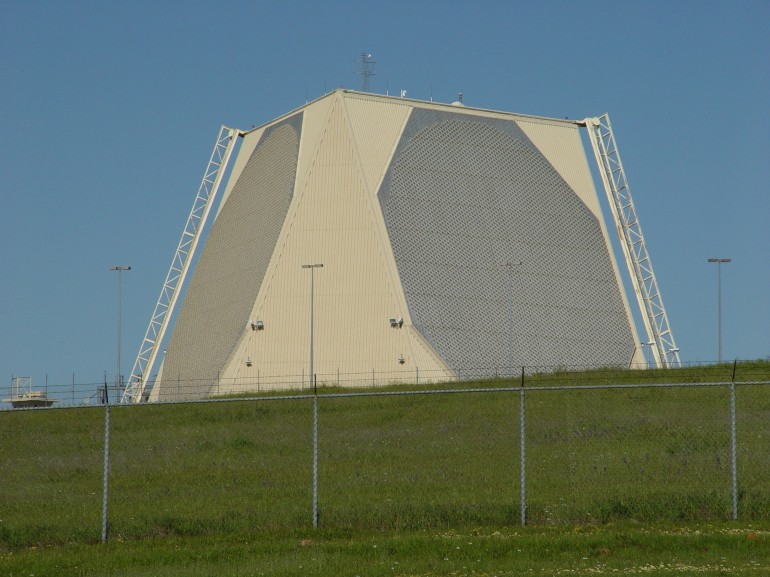
\includegraphics[height=2.7cm]{PhasedArrayRadar}\hspace*{0.2cm}
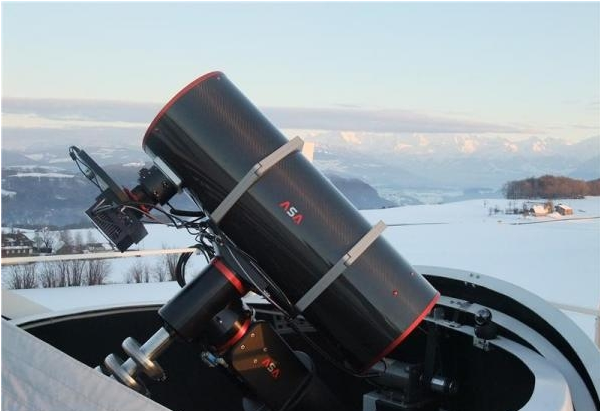
\includegraphics[height=2.7cm]{TelescopeTrackingSats}\hspace*{0.2cm}
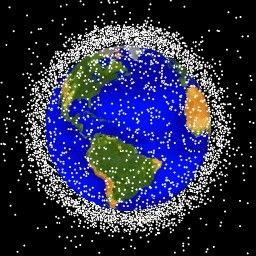
\includegraphics[height=2.7cm]{SatDots}}
\centerline{\scriptsize\selectfont
\hspace*{0.6cm}Phased Array Radar\hspace*{1.7cm} Satellite Tracking Telescope\hspace*{1.0cm} Space Object Illustration}
\end{frame}


\begin{frame}
\frametitle{Introduction}


\begin{itemize}
\item Data association
	\begin{itemize}
	\item Several techniques have been applied to associate measurements with objects
	\item This research focuses on recursive data association techniques that obtain new satellite estimations based on prior estimations and current measurements, not measurements over a long time period--more computationally expensive
	\item \Emph{Hard decision} data association techniques like the nearest neighbor filter \Emph{completely associate} measurements to object estimates, even if there is a nonzero probability that this association is wrong, which can be detrimental to the estimation
	\item \Emph{Soft decision} data association techniques update the satellite tracks with measurements in a \Emph{weighted fashion} based on the probability of association, but often leads to an increase in estimate uncertainties and coalescence of the estimates
	\end{itemize}
\end{itemize}

\end{frame}

\begin{frame}
\frametitle{Introduction}


\begin{itemize}
\item The Joint Probabilistic Data Association Filter (JPDAF)
	\begin{itemize}
	\item Well-known recursive data association technique
	\item The probabilities of association between measurements and objects serve as weighting factors during the measurement update portion of the filter
	\item Designed for linear systems, but easily extended to nonlinear systems if the linearized dynamics are accurate% in the time period between measurement updates
	\end{itemize}
\item The JPDAF suffers from two issues addressed in this paper:
\begin{enumerate}
\item The Kalman gain, which normally minimizes the uncertainty of estimates of individual tracks, is applied but does \Emph{not} minimize the uncertainty of the satellite states with the JPDAF
\item When measurements are shared among multiple objects, the object \Emph{estimates} tend to come together, known as \Emph{coalescence}
\end{enumerate}
\item To solve these problems, we derive the minimum uncertainty JPDAF (MUJPDAF) and the coalescence-avoiding optimal JPDAF (C-JPDAF) and perform numerous simulations to show the benefits and drawbacks of each approach
\end{itemize}

\end{frame}


\section*{}
\subsection*{II. MUJPDAF Problem Formulation}


\begin{frame}
\frametitle{Flow Update}

\begin{itemize}
\item The $i$-th linear stochastic discrete-time system is described by
\begin{align}
x_{i_{k}} & = F_{i_{k-1}} x_{i_{k-1}} + w_{i_{k}},\label{eqn:xkp}\\
z_{i_k} & = H_ix_{i_k} + v_{i_k}
\end{align}
\item Gaussian distributions for the $x_{i_0} \sim \mathcal{N}[\bar x_{i_0}, P_{i_0}]$
\item Zero-mean, mutually independent, white Gaussian noise sequences for the process noise $w_{i_k} \sim \mathcal{N}[0,Q_{i_k}]$ and measurement noise $v_{i_k} \sim \mathcal{N}[0,R_{i_k}]$
\item A priori state covariance
\begin{align}
P_{i_{k}}^- = F_{i_{k-1}} P_{i_{k-1}}^+ F_{i_{k-1}}^T + Q_{i_{k}}
\end{align}
\end{itemize}

\end{frame}

\begin{frame}
\frametitle{Measurement Update}

\begin{itemize}
\item The measurement prediction of the $i$-th estimate $\hat z_i = H_i\hat x_{i}^-$ (linear) or $\hat z_i = h_i(\hat x_{i}^-)$ where $H_i=\deriv{h_i}{x_i}\bigg|_{x_i=\hat x_{i}^-}$ (nonlinear) is compared with the $j$-th measurement to obtain the innovations
\begin{align}
e_{ij} = z_j - \hat z_i\ \ \forall\ i,j
\end{align}
such that the $i$-th covariance matrix is
\begin{align}
S_{i}=H_{i}P_{i}^{-}H_{i}^T+R_{i}=\mathrm{E}[e_{i}e_i^{T}]
\end{align}
\item Measurement origination model based on the "Cheap JPDAF" to obtain the probability that the $i$-th estimate is associated with the $j$-th measurement
\begin{align}
G_{ij}&=\frac1{\sqrt{\det{S_{i}}}}\exp{\{-\frac12e_{ij}^TS_{i}^{-1}e_{ij}\}},
\quad
\mathcal{S}_{ti}=\sum\limits_{j\in J}G_{ij}, 
\quad 
\mathcal{S}_{ri}=\sum\limits_{i\in I}G_{ij},
\\
\beta_{ij}&=\frac{G_{ij}}{\mathcal{S}_{ti}+\mathcal{S}_{ri}-G_{ij}+B}
\end{align}
\end{itemize}

\end{frame}

\begin{frame}
\frametitle{Measurement Update}

\begin{itemize}
\item A posteriori state is
\begin{align}
\hat x^+_{i}=&\ \hat x^-_{i}+K_{i}{\bf{e}}_{i}
\end{align}
where the gain matrix $K_i$ is chosen to minimize the trace of the covariance matrix $P^+_{i}$ where
\begin{align}
P^c_i=&\ (I-K_iH_i)P^-_i(I-K_iH_i)^T+K_iR_iK_i^T,
\\
\tilde P_i=&\ K_i\parenth{{\sum\limits_{j} \beta_{ij}e_{ij}e_{ij}^T-{\bf{e}}_{i}}{\bf{e}}_{i}^T}K_{i}^T,
\\
P^+_{i}=&\ \beta_{0,i}P^-_{i}+(1-\beta_{0,i})P_i^c+\tilde P_i \label{eqn:PostCovBasic}
\end{align}
\item However, the Kalman gain $K_{i,Kalman}=P^-_iH_i^TS_i^{-1}$ is \Emph{not} guaranteed to minimize $\tr{P^+_{i}}$ unless $\tilde P_i=0$, even though it is \Emph{widely used with the JPDAF}
\end{itemize}

\end{frame}

\begin{frame}
\frametitle{Measurement Update}

\begin{itemize}
\item We can rewrite \refeqn{PostCovBasic} as 
\begin{align}
P^+_i&=P^-_{i}-(1-\beta_{0,i})(K_iH_iP^-_i+P^-_iH_i^TK_i^T)
+K_iE_iK_i^T,\label{eqn:CovExpanded}
\\
E_i=&\ (1-\beta_{0,i})S_i+{\sum\limits_{j} \beta_{ij}e_{ij}e_{ij}^T-{\bf{e}}_{i}}{\bf{e}}_{i}^T
\end{align}
\item Then, we choose the gain $K_i$ that minimizes $\tr{P^+_{i}}$ as
\begin{align}
K_i&=(1-\beta_{0,i})P^-_iH_i^TE_i^{-1},\label{eqn:GainK}
\end{align}
such that
\begin{align}
P^+_{i}=&P^-_{i}-K_iE_iK_i^T, \quad \mbox{or equivalently}\label{eqn:JPDAFPostCovSymmetricUpdate}
\\
P^+_{i}=&\left(I-(1-\beta_{0,i})K_iH_i\right)P^-_i\label{eqn:JPDAFPostCovSimpleUpdate}
\end{align}
\end{itemize}

\end{frame}











\section*{}
\subsection*{II. MUJPDAF Numerical Examples}


\begin{frame}
\frametitle{Numerical Problem Formulation}

\begin{itemize}
\item Let $\vec r=\begin{bmatrix}x_1 & x_2 & x_3\end{bmatrix}^T$ be the position vector of the $i$-th satellite represented with respect to the Earth-Centered Inertial (ECI) frame such that $\vec x=\begin{bmatrix}\vec r^T & \dot{\vec r}^T\end{bmatrix}^T\in\Re^6$
\item The nonlinear equation of motion is
\begin{align}
\ddot{\vec r}&=-\frac{\mu}{r^3}\vec r=-\mu(\vec r^T\vec r)^{-\frac32}\vec r
\end{align}
\item The linearized equation is given by
\begin{align}
\begin{bmatrix}
\delta\dot{\vec r} \\ \delta\ddot{\vec r}
\end{bmatrix}
%\delta\dot{\vec x}
=
\begin{bmatrix}
0_{3\times3} & I_{3\times3} \\
\mu\left[3\vec r({\vec r}^T\vec r)^{-\frac52}{\vec r}^T-({\vec r}^T\vec r)^{-\frac32}I_{3\times3}\right] & 0_{3\times3}
\end{bmatrix}
\begin{bmatrix}
\delta\vec r \\ \delta\dot{\vec r}
\end{bmatrix}
\end{align}
\item The ground-based sensor is situated on the equator such that
\begin{align}
x_s=R_E
\begin{bmatrix}
\cos\frac{2\pi t}T & \sin\frac{2\pi t}T & 0 & -\frac{2\pi t}T\sin\frac{2\pi t}T  & \frac{2\pi t}T\cos\frac{2\pi t}T & 0
\end{bmatrix}^T
\end{align}
\end{itemize}

\end{frame}

\begin{frame}
\frametitle{Scenario A1: Comparison of the JPDAF and MUJPDAF with two LEO satellites in close proximity}


\begin{itemize}
\item Two satellites pass nearby with large initial uncertainties
\item Initial conditions:
\begin{align}
x_{1,A1}&=x_{ref,A1}+x_{pert,A1}, \quad x_{2,A1}=x_{ref,A1}-x_{pert,A1},\nonumber
\\
x_{ref,A1}&=\begin{bmatrix}7000 & 0 & 1000 & 0 & 7.546 & 0\end{bmatrix}^T,
\\
x_{pert,A1}&=\begin{bmatrix}
0.2 & 0 & 0 & 0 & -0.105 & 0
\end{bmatrix}^T\nonumber
\end{align}
\item Range, range-rate, topocentric right-ascension and declination measurements are used
\end{itemize}


\end{frame}

\begin{frame}
\frametitle{Scenario A1: Comparison of the JPDAF and MUJPDAF with two LEO satellites in close proximity}


\begin{itemize}
\item A1b: more uncertainty in position
\item A1d: more uncertainty in angular measurements
\end{itemize}

\begin{figure}
\centerline{
	\subfigure[\;Case A1: JPDAF]
		{\hspace*{0.\columnwidth}\includegraphics[width=0.3\columnwidth]{A1JPDAF.pdf}}
	\subfigure[\;Case A1b: JPDAF]
		{\hspace*{0.\columnwidth}\includegraphics[width=0.3\columnwidth]{A1bJPDAF.pdf}}
	\subfigure[\;Case A1d: JPDAF]
		{\hspace*{0.\columnwidth}\includegraphics[width=0.3\columnwidth]{A1dJPDAF.pdf}}
}
\centerline{
	\subfigure[\;Case A1: MUJPDAF]
		{\hspace*{0.\columnwidth}\includegraphics[width=0.3\columnwidth]{A1MUJPDAF.pdf}}
	\subfigure[\;Case A1b: MUJPDAF]
		{\hspace*{0.\columnwidth}\includegraphics[width=0.3\columnwidth]{A1bMUJPDAF.pdf}}
	\subfigure[\;Case A1d: MUJPDAF]
		{\hspace*{0.\columnwidth}\includegraphics[width=0.3\columnwidth]{A1dMUJPDAF.pdf}}
}
\caption{}
\end{figure}

\end{frame}







\begin{frame}
\frametitle{Scenario A2: Comparison of the JPDAF and MUJPDAF with two near-GEO satellites in close proximity}


\begin{itemize}
\item One satellite is on a geostationary orbit while the other has the same state and a small $z$-component
\item Initial conditions:
\begin{align}
x_{1,A2}&=\begin{bmatrix}r_{GEO} & 0 & 0 & 0 & \sqrt{\frac{\mu}{r_{GEO}}}, & 0\end{bmatrix}^T,\nonumber
\\
x_{2,A2}&=x_{1,A2}+\begin{bmatrix}
0 & 0 & -1 & 0 & 0 & 4\times10^{-4}
\end{bmatrix}^T\nonumber
\end{align}
\item Topocentric right-ascension and declination measurements are used
\end{itemize}


\end{frame}

\begin{frame}
\frametitle{Scenario A2: Comparison of the JPDAF and MUJPDAF with two near-GEO satellites in close proximity}


\begin{itemize}
\item A2a: more uncertainty in position
\item A2b: more uncertainty in velocity
\end{itemize}

\begin{figure}
\centerline{
	\subfigure[\;Case A2: JPDAF]
		{\hspace*{0.\columnwidth}\includegraphics[width=0.3\columnwidth]{A2JPDAF.pdf}}
	\subfigure[\;Case A2a: JPDAF]
		{\hspace*{0.\columnwidth}\includegraphics[width=0.3\columnwidth]{A2aJPDAF.pdf}}
	\subfigure[\;Case A2b: JPDAF]
		{\hspace*{0.\columnwidth}\includegraphics[width=0.3\columnwidth]{A2bJPDAF.pdf}}
}
\centerline{
	\subfigure[\;Case A2: MUJPDAF]
		{\hspace*{0.\columnwidth}\includegraphics[width=0.3\columnwidth]{A2MUJPDAF.pdf}}
	\subfigure[\;Case A2a: MUJPDAF]
		{\hspace*{0.\columnwidth}\includegraphics[width=0.3\columnwidth]{A2aMUJPDAF.pdf}}
	\subfigure[\;Case A2b: MUJPDAF]
		{\hspace*{0.\columnwidth}\includegraphics[width=0.3\columnwidth]{A2bMUJPDAF.pdf}}
}
\caption{}
\end{figure}

\end{frame}

























\section*{}
\subsection*{III. C-JPDAF Problem Formulation}


\begin{frame}
\frametitle{Similarity Measure}

\begin{itemize}
\item Coalescence is well-known to occur when measurements are shared, which happens when the similarity among estimates is high
\item Illustration of similarity in a single dimension:
\begin{figure}
\centerline{
		{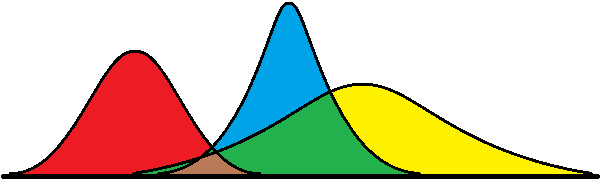
\includegraphics[width=.7\columnwidth]{GaussianDistOverlap1D.png}}
	}
\end{figure}
\item Define the similarity measure between an arbitrary number of Gaussian distributions:
\begin{align}
\zeta=\sum\limits_{p,q\in I,p\neq q}\exp \{-a(\hat y_{p}- \hat y_{q})^T({\mathbf P}_{p}
+{\mathbf P}_{q})^{-1}(\hat y_{p}-\hat y_{q})\}
\end{align}
where $\hat y_i$ has an uncertainty described by the covariance matrix ${\mathbf P}_{i}$
\end{itemize}

\end{frame}

\begin{frame}
\frametitle{Coalescence-Avoiding Gain Matrix}

\begin{itemize}
\item Main idea: choose the gain matrix $K_i$ to minimize a weighted sum of uncertainty and similarity
\item Cost function $\mathbf{J}\in\Re$ to minimize:
\begin{align}
\mathbf{J}=J_P+cJ_S,\quad J_P=\sum\limits_{i}\tr{P^+_i}, \quad J_S&=\sum\limits_{p,q\in I,p\neq q}\exp (-au_{pq}),
\end{align}
for $a,c>0$.
\item Nonlinear equations do not yield a closed-form solution
\end{itemize}
\begin{figure}
\setlength{\unitlength}{0.05\columnwidth}
\centerline{\footnotesize\selectfont
\begin{picture}(8.5,7.3)(-0.5,-0.8)
\put(-0.5,3){\rotatebox{90}{Cost}}
\put(0,0){\includegraphics[width=0.4\columnwidth]{ECC14_fig1.pdf}}
\put(5.0,1.1){\shortstack[c]{Uncertainty\\ cost: $J_P$}}
\put(5.7,2.3){\shortstack[c]{Similarity\\ cost: $J_S$}}
\put(2.2,4.0){\shortstack[c]{Weighted sum:\\ $\mathbf{J}=J_P+cJ_S$}}
\put(4.98,0.78){\circle*{0.1}}
\put(2.48,1.57){\circle*{0.1}}
\put(4.8,-0.4){$K_{MUJPDAF}$}
\put(2.3,-0.4){$K_{C-JPDAF}$}
\end{picture}
}
\end{figure}

\end{frame}







\section*{}
\subsection*{IV. C-JPDAF Numerical Examples}


\begin{frame}
\frametitle{Scenario B1: Comparison of the JPDAF, MUJPDAF, and C-JPDAF with three LEO satellites in close proximity}


\begin{itemize}
\item Three satellites have nearly the same initial state except for a small perturbation in the $x$-direction
\item Initial conditions:
\begin{align}
\begin{split}
x_{1,B1}&=x_{ref,B1}+x_{pert,B1}, \quad x_{2,B1}=x_{ref,B1}-x_{pert,B1}, \quad x_{3,B1}=x_{ref,B1},
\\
x_{ref,B1}&=\begin{bmatrix}7000 & 0 & 0 & 0 & 7.546 & 0\end{bmatrix}^T,\nonumber
\\
x_{pert,B1}&=\begin{bmatrix}
0.025 & 0 & 0 & 0 & 0 & 0
\end{bmatrix}^T\nonumber
\end{split}
\end{align}
\item Range, range-rate, topocentric right-ascension and declination measurements are used
\item B1c: position and velocity are more uncertain
\item B1f: range-rate measurement is more uncertain
\end{itemize}


\end{frame}

\begin{frame}
\frametitle{Scenario B1: JPDAF, MUJPDAF, and C-JPDAF in LEO}


%\begin{itemize}
%\item B1b: more uncertainty in measurement range rate
%\item B1d: more uncertainty in angular measurements
%\end{itemize}
\begin{figure}
%\vspace*{-0.3cm}
\centerline{
	\subfigure[\;B1: JPDAF]
		{\hspace*{0.\columnwidth}\includegraphics[width=0.23\columnwidth]{B1JPDAF.pdf}}
	\subfigure[\;B1: MUJPDAF]
		{\hspace*{0.\columnwidth}\includegraphics[width=0.23\columnwidth]{B1MUJPDAF.pdf}}
	\subfigure[\;B1: C-JPDAF]
		{\hspace*{0.\columnwidth}\includegraphics[width=0.23\columnwidth]{B1C-JPDAF.pdf}}
	}
%\vspace*{-0.2cm}
\centerline{
	\subfigure[\;B1c: JPDAF]
		{\hspace*{0.\columnwidth}\includegraphics[width=0.23\columnwidth]{B1cJPDAF.pdf}}
	\subfigure[\;B1c: MUJPDAF]
		{\hspace*{0.\columnwidth}\includegraphics[width=0.23\columnwidth]{B1cMUJPDAF.pdf}}
	\subfigure[\;B1c: C-JPDAF]
		{\hspace*{0.\columnwidth}\includegraphics[width=0.23\columnwidth]{B1cC-JPDAF.pdf}}
	}
%\vspace*{-0.2cm}
\centerline{
	\subfigure[\;B1f: JPDAF]
		{\hspace*{0.\columnwidth}\includegraphics[width=0.23\columnwidth]{B1fJPDAF.pdf}}
	\subfigure[\;B1f: MUJPDAF]
		{\hspace*{0.\columnwidth}\includegraphics[width=0.23\columnwidth]{B1fMUJPDAF.pdf}}
	\subfigure[\;B1f: C-JPDAF]
		{\hspace*{0.\columnwidth}\includegraphics[width=0.23\columnwidth]{B1fC-JPDAF.pdf}}
	}
\caption{}
\end{figure}








\end{frame}







\begin{frame}
\frametitle{Scenario B2: Comparison of the JPDAF, MUJPDAF, and C-JPDAF with two GEO satellites in close proximity}


\begin{itemize}
\item Two satellites in a geostationary orbit are offset by a very small phase shift
\item Initial conditions:
\begin{align}
\begin{split}
f_{GEO,r}(\theta)&=\begin{bmatrix}r_{GEO}\cos\theta & r_{GEO}\sin\theta & 0\end{bmatrix}^T,
\\
\quad f_{GEO,\dot r}(\theta)&=\begin{bmatrix}\sqrt{\frac{\mu}{r_{GEO}}}\cos(90^\circ+\theta) & \sqrt{\frac{\mu}{r_{GEO}}}\sin(90^\circ+\theta) & 0\end{bmatrix}^T
\\
f_{GEO}(\theta)&=\begin{bmatrix}f_{GEO,r} & f_{GEO,\dot r}\end{bmatrix}^T,
\\
x_{1,B2}&=f_{GEO}(0^\circ), \quad x_{2,B2}=f_{GEO}({10^{-4}}^\circ)
\end{split}\nonumber
\end{align}
\item Topocentric right-ascension and declination measurements are used
\item B2b: velocity is more uncertain
\item B2d: angle measurements are more uncertain
\end{itemize}


\end{frame}

\begin{frame}
\frametitle{Scenario B2: JPDAF, MUJPDAF, and C-JPDAF in GEO}


\begin{figure}
%\vspace*{-0.3cm}
\centerline{
	\subfigure[\;B2: JPDAF]
		{\hspace*{0.\columnwidth}\includegraphics[width=0.23\columnwidth]{B2JPDAF.pdf}}
	\subfigure[\;B2: MUJPDAF]
		{\hspace*{0.\columnwidth}\includegraphics[width=0.23\columnwidth]{B2MUJPDAF.pdf}}
	\subfigure[\;B2: C-JPDAF]
		{\hspace*{0.\columnwidth}\includegraphics[width=0.23\columnwidth]{B2C-JPDAF.pdf}}
	}
\centerline{
	\subfigure[\;B2b: JPDAF]
		{\hspace*{0.\columnwidth}\includegraphics[width=0.23\columnwidth]{B2bJPDAF.pdf}}
	\subfigure[\;B2b: MUJPDAF]
		{\hspace*{0.\columnwidth}\includegraphics[width=0.23\columnwidth]{B2bMUJPDAF.pdf}}
	\subfigure[\;B2b: C-JPDAF]
		{\hspace*{0.\columnwidth}\includegraphics[width=0.23\columnwidth]{B2bC-JPDAF.pdf}}
	}
\centerline{
	\subfigure[\;B2d: JPDAF]
		{\hspace*{0.\columnwidth}\includegraphics[width=0.23\columnwidth]{B2dJPDAF.pdf}}
	\subfigure[\;B2d: MUJPDAF]
		{\hspace*{0.\columnwidth}\includegraphics[width=0.23\columnwidth]{B2dMUJPDAF.pdf}}
	\subfigure[\;B2d: C-JPDAF]
		{\hspace*{0.\columnwidth}\includegraphics[width=0.23\columnwidth]{B2dC-JPDAF.pdf}}
	}
\caption{}
\end{figure}

\end{frame}

\begin{frame}
\frametitle{Computation Time}

\begin{center}
\resizebox{0.66\columnwidth}{!}{
\begin{threeparttable}[h]
\caption{B1 Scenarios} \label{tab:B1}
\begin{tabularx}{1.16\columnwidth}
{
>{$}c<{$} |
*{3}{>{$}c<{$}} |
*{3}{>{$}c<{$}}
}
\toprule
\multirow{2}{*}{Case} & \multicolumn{3}{c}{\multirow{1}{*}{RMS Position Error (km)}} & \multicolumn{3}{c}{\multirow{1}{*}{Time (sec)}} \\
 & \multirow{1}{*}{JPDAF} & \multirow{1}{*}{MUJPDAF} & \multirow{1}{*}{C-JPDAF} & \multirow{1}{*}{JPDAF} & \multirow{1}{*}{MUJPDAF} & \multirow{1}{*}{C-JPDAF}
\\
\midrule
B1   	& 0.14432 & 0.091133 & 0.057312 & 1.736272 & 1.670539 & 101.000529 \\
B1a 	& 0.14432 & 0.091134 & 0.057307 & 1.689807 & 1.726980 & 100.988662 \\
B1b 	& 0.14694 & 0.094506 & 0.055145 & 1.673762 & 1.678786 & 100.855376 \\
B1c 	& 0.14693 & 0.094507 & 0.055136 & 1.675486 & 1.669083 & 100.907850 \\
B1d 	& 0.14400 & 0.088933 & 0.058911 & 1.663424 & 1.660136 & 102.606102 \\
B1e 	& 0.14408 & 0.090823 & 0.059919 & 1.673660 & 1.666829 & 100.278073 \\
B1f 	& 0.14436 & 0.091212 & 0.064299 & 1.732541 & 1.721413 & 98.672870 \\
\bottomrule
\end{tabularx}
\end{threeparttable}
}
\end{center}

\begin{center}
\resizebox{0.8\columnwidth}{!}{
\begin{threeparttable}[h]
\caption{B2 Scenarios} \label{tab:B2}
\begin{tabularx}{1.35\columnwidth}
{
>{$}c<{$} |
*{3}{>{$}c<{$}} |
*{3}{>{$}c<{$}}
}
\toprule
\multirow{2}{*}{Case} & \multicolumn{3}{c}{\multirow{1}{*}{RMS Angular Error (rad)}} & \multicolumn{3}{c}{\multirow{1}{*}{Time (sec)}} \\
 & \multirow{1}{*}{JPDAF} & \multirow{1}{*}{MUJPDAF} & \multirow{1}{*}{C-JPDAF} & \multirow{1}{*}{JPDAF} & \multirow{1}{*}{MUJPDAF} & \multirow{1}{*}{C-JPDAF}
\\
\midrule
B2   	& 1.1112\times10^{-6} & 9.4780\times10^{-7} & 5.6708\times10^{-7} & 1.149378 & 1.119439 & 34.318254 \\
B2a 	& 1.1112\times10^{-6} & 9.4779\times10^{-7} & 5.6347\times10^{-7} & 1.154256 & 1.150072 & 34.758609 \\
B2b 	& 1.1306\times10^{-6} & 9.8287\times10^{-7} & 5.7387\times10^{-7} & 1.126598 & 1.132463 & 35.327683 \\
B2c 	& 1.1306\times10^{-6} & 9.8286\times10^{-7} & 5.6435\times10^{-7} & 1.118436 & 1.131690 & 34.817179 \\
B2d 	& 1.1115\times10^{-6} & 9.5439\times10^{-7} & 5.6136\times10^{-7} & 1.113892 & 1.116399 & 35.213445 \\
\bottomrule
\end{tabularx}
\end{threeparttable}
}
\end{center}



\end{frame}

\section*{}
\subsection*{IV. Conclusions}

\begin{frame}
\frametitle{Conclusions}

\begin{itemize}
\item The Kalman gain is not guaranteed to minimize the state uncertainty generated by the JPDAF
\begin{itemize}
\item This motivates the derivation of the minimum uncertainty JPDAF, designed to account for all parts of the state covariance by changing the gain matrix (not Kalman), derived as a research contribution
\item Numerous simulations show that the MUJPDAF experiences smaller RMS errors and covariances in \Emph{every} simulated scenario
\item The computation is nearly identical between the algorithms
\end{itemize}
\item Both the JPDAF and MUJPDAF experience coalescence
\begin{itemize}
\item Research contribution: the C-JPDAF, which systematically removes coalescence from the soft decision techniques
\item Similar to the derivation of the MUJPDAF, we choose a gain that minimizes a weighted sum of uncertainty and similarity
\item In many cases, this leads to improved accuracy of the estimation in exchange for a greater computational load
\end{itemize}
\item Future work
\begin{itemize}
\item Determine systematic way of choosing weighting parameters for the C-JPDAF
\item Solve a sub-optimal solution for the C-JPDAF to decrease its computational load to a practical level
\end{itemize}
\end{itemize}

\end{frame}



\end{document}






















